\documentclass[a4paper,12pt]{extarticle}
\usepackage[margin=1.5cm]{geometry}
\usepackage[russian]{babel}
\usepackage[utf8]{inputenc}
\usepackage{tikz}
\usepackage{hedmaths}

\renewcommand{\small}{\fontsize{12pt}{14.4pt}\selectfont}
\usepackage{caption}
\DeclareCaptionLabelFormat{figure}{Рисунок #2}
\DeclareCaptionLabelFormat{table}{Таблица #2}
\DeclareCaptionLabelSeparator{sep}{~---~}
\captionsetup{labelsep=sep,justification=centering,font=small}
\captionsetup[figure]{labelformat=figure}
\captionsetup[table]{labelformat=table}

\usepackage{titlesec}
\titleformat{\section}
    {\centering\normalsize}
    {\thesection}
    {1em}{}
\titleformat{\subsection}
    {\centering\normalsize}
    {\thesubsection}
    {1em}{}
\titleformat{\subsubsection}
    {\centering\normalsize}
    {\thesubsubsection}
    {1em}{}

\titlespacing*{\section}{\parindent}{*4}{*1}
\titlespacing*{\subsection}{\parindent}{*4}{*1}
\titlespacing*{\subsubsection}{\parindent}{*4}{*1}

\renewcommand{\tan}{\mathrm{tg\,}}
\renewcommand{\baselinestretch}{1.5}

\parindent=1.25cm
\usepackage{enumitem}
\makeatletter
\AddEnumerateCounter{\asbuk}{\@asbuk}{м)}
\makeatother
\setlist{nosep,wide}

\tolerance=10000

\begin{document}
	\begin{titlepage}
        \begin{center}
          Министерство образования и науки Российской Федерации \\
          Федеральное государственное бюджетное образовательное \\
          учреждение высшего профессионального образования \\
          <<Волгоградский государственный технический университет>> \\
          Факультет электроники и вычислительной техники\\
          Кафедра <<Физика>>
        \end{center}
        \vspace{9em}
        \begin{center}
          \large
          Семестровая работа
		  по дисциплине\\
		  <<Электродинамика СВЧ>>\\
        \end{center}
        \vspace{5em}
        \begin{flushright}
          \begin{minipage}{.40\textwidth}
            Выполнил:\\
            студент группы Ф-1н\\
            Абдрахманов В. Л.\\
            \vspace{1em}\\
            Проверил:\\
            к.ф.-м.н., доцент\\
            Грецов М. В.
          \end{minipage}
        \end{flushright}
        \vspace{\fill}
        \begin{center}
          Волгоград, \the\year
        \end{center}
    \end{titlepage}
    \setcounter{page}{2}
	\emph{
	Прямоугольный волновод 23\(\times\)10 мм, закороченный в сечении z=0 возбуждается тонким штырём длины \( l \)= 8 мм, введённым через широкую стенку параллельно узкой стенке и расположенным в \( z_0 \) = 15 мм, \( x_0 \) = 10 мм. Амплитуда тока в штыре \( I_0 \)= 2 А, частота \( f \) = 17 ГГц. Рассчитать спектр типов волн и их амплитудные коэффициенты (отношение максимальной амплитуды к минимальной 20, моды с меньшей амплитудой не учитывать), а также рассчитать распределение мощности в поперечном сечении волновода и мощность, переносимую в волноводе.
	}
	\vspace*{1cm}

	Для начала, определим какие вообще волны могут распространяться в волноводе на этой частоте:
	\[
		\frac{m^2}{a^2} + \frac{n^2}{b^2} < \left(\frac{2f}{c}\right)^2,
	\]
	\[
		\frac{m^2}{\left(\frac{2fa}{c}\right)^2} + \frac{n^2}{\left(\frac{2fb}{c}\right)^2} < 1.
	\]

	Возможным модам будут удовлетворять точки с целочисленными координатами внутри четверти эллипса с полуосями \( 2fa/c = 2.61 \) и \( 2fb/c = 1.13 \):

	\begin{figure}[h]
		\center
		\begin{tikzpicture}[scale=3]
			\fill[fill=blue!20,thick,draw=black] (2.61,0) arc (0:90:2.61 and 1.13) -- (0,0) -- (2.61,0) -- cycle;
			\draw (-0.2,0) -- (2.7, 0);
			\draw (0,-0.2) -- (0, 1.3);

			\fill[black] (0,1) circle (0.03) node[left]{$(0,1)$};
			\fill[black] (1,1) circle (0.03) node[below]{$(1,1)$};
			\draw (2,1) circle (0.03) node[right]{$(2,1)$};
			\fill[black] (1,0) circle (0.03) node[below]{$(1,0)$};
			\fill[black] (2,0) circle (0.03) node[below]{$(2,0)$};
		\end{tikzpicture}
	\end{figure}

	Итого 5 типов волн: 4 H-волны и E-волна. Перенумеруем их:
	\begin{table}[h]
		\center
		\begin{tabular}{|c|c|c|c|c|c|}\hline
			Волна & $H_{10}$ & $H_{20}$ & $H_{01}$ & $H_{11}$ & $E_{11}$ \\ \hline
			$k$ & 1 & 2 & 3 & 4 & 5 \\ \hline
		\end{tabular}
	\end{table}

	Теперь рассмотрим их возбуждение током. Геометрия системы имеет вид

	\begin{figure}[h]
		\center
		\begin{tikzpicture}[scale=0.15]
			\draw[very thick] (25, 10) -- (0, 10) -- (0, 0) -- (25, 0);
			\draw[thick] (15, 0) -- (15, 8);
			\draw[->] (-4, -3) -- (30, -3);
			\draw[->] (-3, -4) -- (-3, 13);
			\draw (0, -2.6) -- (0, -3.4) node[below]{$0$};
			\draw (15, -2.6) -- (15, -3.4) node[below]{$z_0$};
			\node[below] at (30,-3.4) {$z$};

			\draw (-2.6,0) -- (-3.4,0) node[left]{$0$};
			\draw (-2.6,8) -- (-3.4,8) node[left]{$l$};
			\node[left] at (-3.4, 13) {$y$};
		\end{tikzpicture} \hfil
		\begin{tikzpicture}[scale=0.15]
			\draw[very thick] (0, 0) rectangle (23, 10);
			\draw[thick] (10, 0) -- (10, 8);
			\draw[->] (-4, -3) -- (25, -3);
			\draw[->] (-3, -4) -- (-3, 13);
			\draw (0, -2.6) -- (0, -3.4) node[below]{$0$};
			\draw (10, -2.6) -- (10, -3.4) node[below]{$x_0$};
			\node[below] at (25,-3.4) {$x$};

			\draw (-2.6,0) -- (-3.4,0) node[left]{$0$};
			\draw (-2.6,8) -- (-3.4,8) node[left]{$l$};
			\node[left] at (-3.4, 13) {$y$};
		\end{tikzpicture}
	\end{figure}

	При возбуждении одним только током коэффициенты Фурье у собственных волн вычисляются следующим образом:
	\[
		A_{\pm k} = \frac{1}{2N_k} \int_V \vec{j}^\text{ст}\cdot\vec{E}_{\mp k} dV = \frac{I_0}{2N_k} \int_0^l \vec{E}_{\mp k}(x_0,y,z_0)\cdot \vec{e}_y dy.
	\]

	Выпишем компоненты \( E \)-волн
	\begin{align*}
		& E_z = E_0\sin\frac{m\pi x}{a}\sin\frac{n\pi y}{b}e^{-ihz},\\
		& H_z = 0,\\
		& E_x = -i\frac{hm\pi}{g_{m,n}^2a}E_0\cos\frac{m\pi x}{a}\sin\frac{n\pi y}{b}e^{-ihz},\\
		& E_y = -i\frac{hn\pi}{g_{m,n}^2b}E_0\sin\frac{m\pi x}{a}\cos\frac{n\pi y}{b}e^{-ihz},\\
		& H_x = -\frac{\omega\eps}{h}E_y = i\frac{\omega\eps n\pi}{g_{m,n}^2b}E_0\sin\frac{m\pi x}{a}\cos\frac{n\pi y}{b}e^{-ihz},\\
		& H_y = \frac{\omega\eps}{h}E_x = -i\frac{\omega\eps m\pi}{g_{m,n}^2a}E_0\cos\frac{m\pi x}{a}\sin\frac{n\pi y}{b}e^{-ihz}.
	\end{align*}

	и \( H \)-волн:
	\begin{align*}
		& E_z = 0,\\
		& H_z = H_0\cos\frac{m\pi x}{a}\cos\frac{n\pi y}{b}e^{-ihz},\\
		& E_x = i\frac{\omega\mu n\pi}{g_{m,n}^2b}H_0\cos\frac{m\pi x}{a}\sin\frac{n\pi y}{b}e^{-ihz},\\
		& E_y = -i\frac{\omega\mu m\pi}{g_{m,n}^2a}H_0\sin\frac{m\pi x}{a}\cos\frac{n\pi y}{b}e^{-ihz},\\
		& H_x = -\frac{h}{\omega\mu}E_y = i\frac{hm\pi}{g_{m,n}^2a}H_0\sin\frac{m\pi x}{a}\cos\frac{n\pi y}{b}e^{-ihz},\\
		& H_y = \frac{h}{\omega\mu}E_x = i\frac{h n\pi}{g_{m,n}^2b}H_0\cos\frac{m\pi x}{a}\sin\frac{n\pi y}{b}e^{-ihz}.
	\end{align*}

	Распределение мощности по поперечному сечению имеет вид
	\begin{align*}
		& \Pi_E = \frac{1}{2}\frac{\omega\eps}{h}\left(|E_x|^2 + |E_y|^2\right) = \\
		& = \frac{1}{2}\frac{\omega\eps h E_0^2}{\left(\frac{\pi^2m^2}{a^2} + \frac{\pi^2n^2}{b^2}\right)^2}\left( \left(\frac{m\pi}{a}\right)^2\cos^2\frac{m\pi x}{a}\sin^2\frac{n\pi y}{b} + \left(\frac{n\pi}{b}\right)^2\sin^2\frac{m\pi x}{a}\cos^2\frac{n\pi y}{b} \right) \\
		& \Pi_H = \frac{1}{2}\frac{h}{\omega\mu}\left(|E_x|^2 + |E_y|^2\right) = \\
		& = \frac{1}{2}\frac{\omega\mu h H_0^2}{\left(\frac{\pi^2m^2}{a^2} + \frac{\pi^2n^2}{b^2}\right)^2}\left( \left(\frac{n\pi}{b}\right)^2\cos^2\frac{m\pi x}{a}\sin^2\frac{n\pi y}{b} + \left(\frac{m\pi}{a}\right)^2\sin^2\frac{m\pi x}{a}\cos^2\frac{n\pi y}{b} \right)
	\end{align*}

	Мощность, переносимая волной:
	\begin{align*}
		& P_E = \frac{ab}{8}\frac{\omega\eps h E_0^2}{\left(\frac{\pi^2m^2}{a^2} + \frac{\pi^2n^2}{b^2}\right)^2}\left( \left(\frac{m\pi}{a}\right)^2 + \left(\frac{n\pi}{b}\right)^2 \right) = \frac{ab}{8}\frac{\omega\eps h E_0^2}{\frac{\pi^2m^2}{a^2} + \frac{\pi^2n^2}{b^2}} \\
		& P_H =
			\frac{ab}{8-4(\delta_{m0}+\delta_{n0})}\frac{\omega\mu h H_0^2}{\frac{\pi^2m^2}{a^2} + \frac{\pi^2n^2}{b^2}}.
	\end{align*}

	Нормы связаны с мощностями соотношением
	\[
		N_k = 2P_{m_k,n_k}.
	\]

	Определим коэффициенты для \( k = \overline{1,4} \):
	\[
		A_{\pm k} = -i\frac{I_0}{2N_k} \int_0^l \frac{\omega\mu m\pi}{g_{m_k,n_k}^2a}H_0\sin\frac{m\pi x_0}{a}\cos\frac{n\pi y}{b}e^{\pm ihz_0}\,dy,
	\]

	\begin{align*}
		& A_{\pm 1} = -i\frac{I_0}{4\frac{ab}{4}\frac{\omega\mu h_1 H_0^2}{g_{10}^2}} \frac{\omega\mu \pi}{g_{10}^2a}H_0\sin\frac{\pi x_0}{a}e^{\pm ih_1z_0}l = -i\frac{I_0}{ab h_1 H_0} \frac{\pi l}{a}\sin\frac{\pi x_0}{a}e^{\pm ih_1z_0},\\
		& A_{\pm 2} = -i\frac{I_0}{ab h_2 H_0} \frac{2\pi l}{a}\sin\frac{2\pi x_0}{a}e^{\pm ih_2z_0},\\
		& A_{\pm 3} = 0,\\
		& A_{\pm 4} = -i\frac{I_0}{4\frac{ab}{8}\frac{\omega\mu h_4 H_0^2}{g_{11}^2}} \frac{\omega\mu \pi}{g_{11}^2a}H_0\sin\frac{\pi x_0}{a}\frac{b}{\pi}\sin\frac{\pi l}{b}e^{\pm ih_4z_0} = -i\frac{2I_0}{ab h_4 H_0} \frac{b}{a}\sin\frac{\pi x_0}{a}\sin\frac{\pi l}{b}e^{\pm ih_4z_0}.
	\end{align*}

	Для \( k = 5 \):
	\[
		A_{\pm 5} =  \pm i\frac{I_0}{4\frac{ab}{8}\frac{\omega\eps h_5 E_0^2}{g_{11}^2}}\frac{h_5\pi}{g_{11}^2b}E_0\sin\frac{\pi x_0}{a}\frac{b}{\pi}\sin\frac{\pi l}{b}e^{\pm ih_5z_0} = \pm i \frac{2I_0}{ab\omega\eps E_0} \sin\frac{\pi x_0}{a}\sin\frac{\pi l}{b}e^{\pm ih_5z_0}.
	\]

	Волны идущие влево полностью отразятся на закоротке. Коэффициенты отражённых волн можно найти из граничных условий на поперечные компоненты электрического поля при \( z=0 \):
	\[
		A_k^r = \begin{cases}
			-A_{-k}, k=\overline{1,4},\\
			A_{-k}, k=5.
		\end{cases}
	\]

	Вдали от штыря справа коэффициенты разложения волны имеют вид
	\[
		B_k = A_k + A_k^r.
	\]

	Подставив конкретный вид, получим
	\begin{align*}
		& B_1 = -i\frac{I_0}{ab h_1 H_0} \frac{\pi l}{a}\sin\frac{\pi x_0}{a}(e^{ih_1z_0}  - e^{-ih_1z_0}) = \frac{2I_0}{ab h_1 H_0} \frac{\pi l}{a}\sin\frac{\pi x_0}{a}\sin(h_1z_0),\\
		& B_2 = \frac{2I_0}{ab h_2 H_0} \frac{2\pi l}{a}\sin\frac{2\pi x_0}{a}\sin(h_2z_0),\\
		& B_4 = \frac{4I_0}{ab h_4 H_0} \frac{b}{a}\sin\frac{\pi x_0}{a}\sin\frac{\pi l}{b}\sin(h_4z_0),\quad
		B_5 = \frac{4I_0}{ab\omega\eps E_0} \sin\frac{\pi x_0}{a}\sin\frac{\pi l}{b}\sin(h_5z_0).
	\end{align*}

	Определим мощности \( P_k \), переносимые волнами:
	\begin{align*}
		P_1 &= \frac{ab}{4}\frac{\omega\mu h_1}{g_{10}^2}\left[\frac{2I_0}{ab h_1} \frac{\pi l}{a}\sin\frac{\pi x_0}{a}\sin(h_1z_0)\right]^2= 
		\frac{\omega\mu I_0^2}{ab h_1}\left[l\sin\frac{\pi x_0}{a}\sin(h_1z_0)\right]^2,\\
		P_2 &= \frac{ab}{4}\frac{\omega\mu h_2}{g_{20}^2}\left[\frac{2I_0}{ab h_2} \frac{2\pi l}{a}\sin\frac{2\pi x_0}{a}\sin(h_2z_0)\right]^2= 
		\frac{\omega\mu I_0^2}{ab h_2}\left[l\sin\frac{2\pi x_0}{a}\sin(h_2z_0)\right]^2,\\
		P_4 &= \frac{ab}{8}\frac{\omega\mu h_4}{g_{11}^2}\left[\frac{4I_0}{ab h_4} \frac{b}{a}\sin\frac{\pi x_0}{a}\sin\frac{\pi l}{b}\sin(h_4z_0)\right]^2 = \frac{2\omega\mu I_0^2}{abh_4g_{11}^2}\left[\frac{b}{a}\sin\frac{\pi x_0}{a}\sin\frac{\pi l}{b}\sin(h_4z_0)\right]^2,\\
		P_5 &= \frac{ab}{8}\frac{\omega\eps h_5}{g_{11}^2} \left[\frac{4I_0}{ab\omega\eps} \sin\frac{\pi x_0}{a}\sin\frac{\pi l}{b}\sin(h_5z_0)\right]^2 =
		\frac{h_5}{g_{11}^2} \frac{2I_0^2}{ab\omega\eps} \left[\sin\frac{\pi x_0}{a}\sin\frac{\pi l}{b}\sin(h_5z_0)\right]^2.
	\end{align*}

	\begin{table}[h]
		\center
		\caption{Спектр волн в волноводе}
		\begin{tabular}{|c|c|c|}\hline
		Тип волны & $h,\text{ м}^{-1}$ & $P,\text{ Вт}$ \\ \hline
		$H_{10}$ & 330 & 410 \\
		$H_{20}$ & 230 & 8,1 \\
		$H_{11}$ & 97 & 25 \\
		$E_{11}$ & 97 & 9,9 \\ \hline
		\end{tabular}
	\end{table}

	Полная мощность, переносимая в волноводе
	\[
		P = P_1 + P_2 + P_4 + P_5 = 450~\text{Вт}.
	\]

	\begin{figure}[h]
		\center
		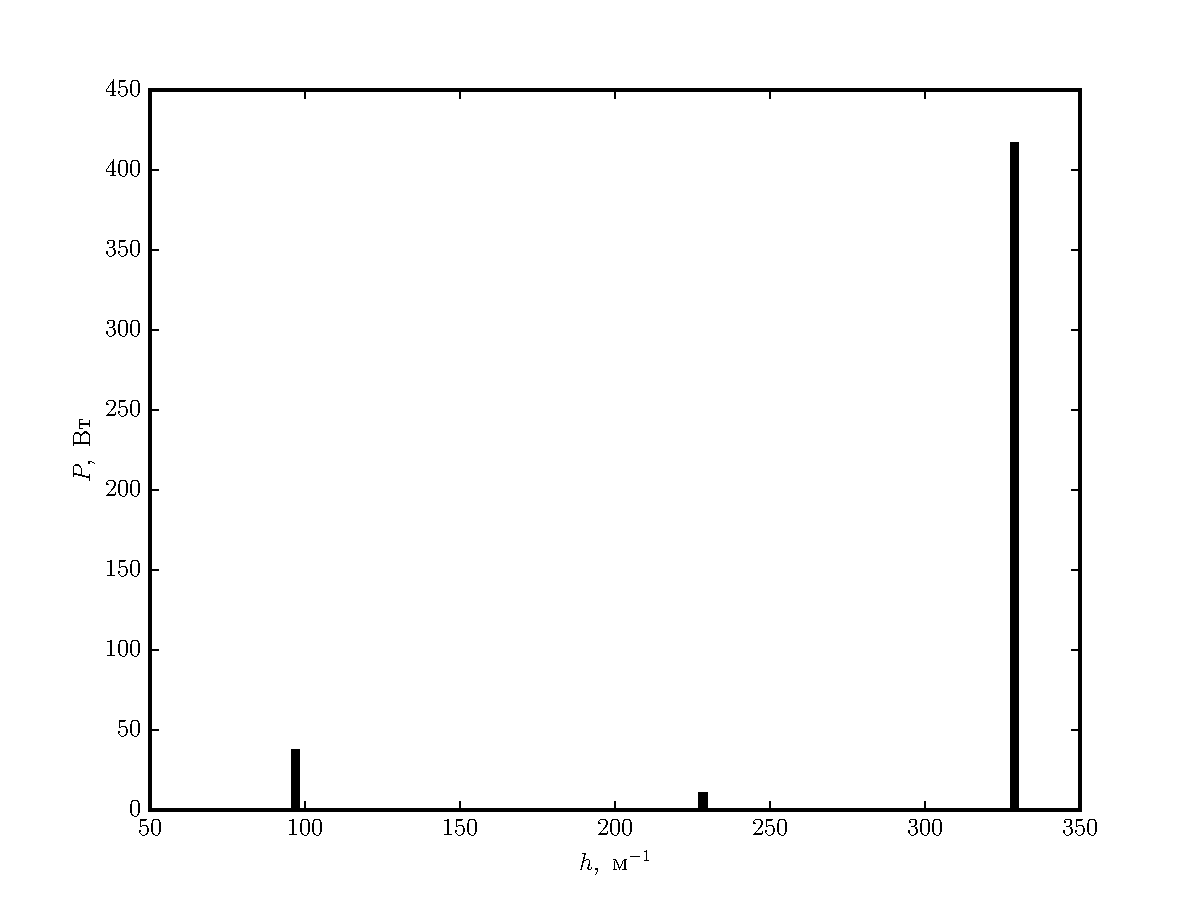
\includegraphics[width=.8\textwidth]{spectrum}
		\caption{Спектральный состав излуения в волноводе}
	\end{figure}
	
	\begin{figure}
		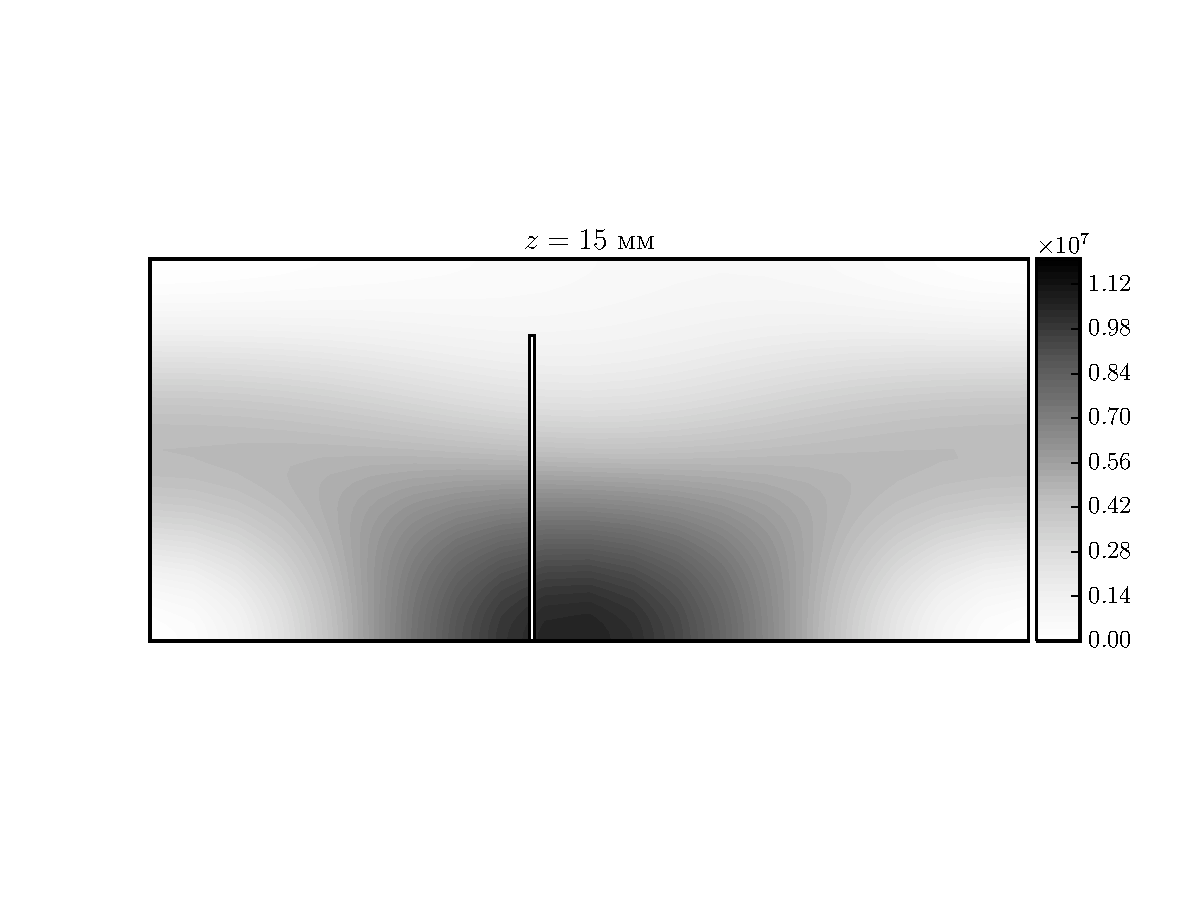
\includegraphics[width=.5\textwidth]{15}\hfil
		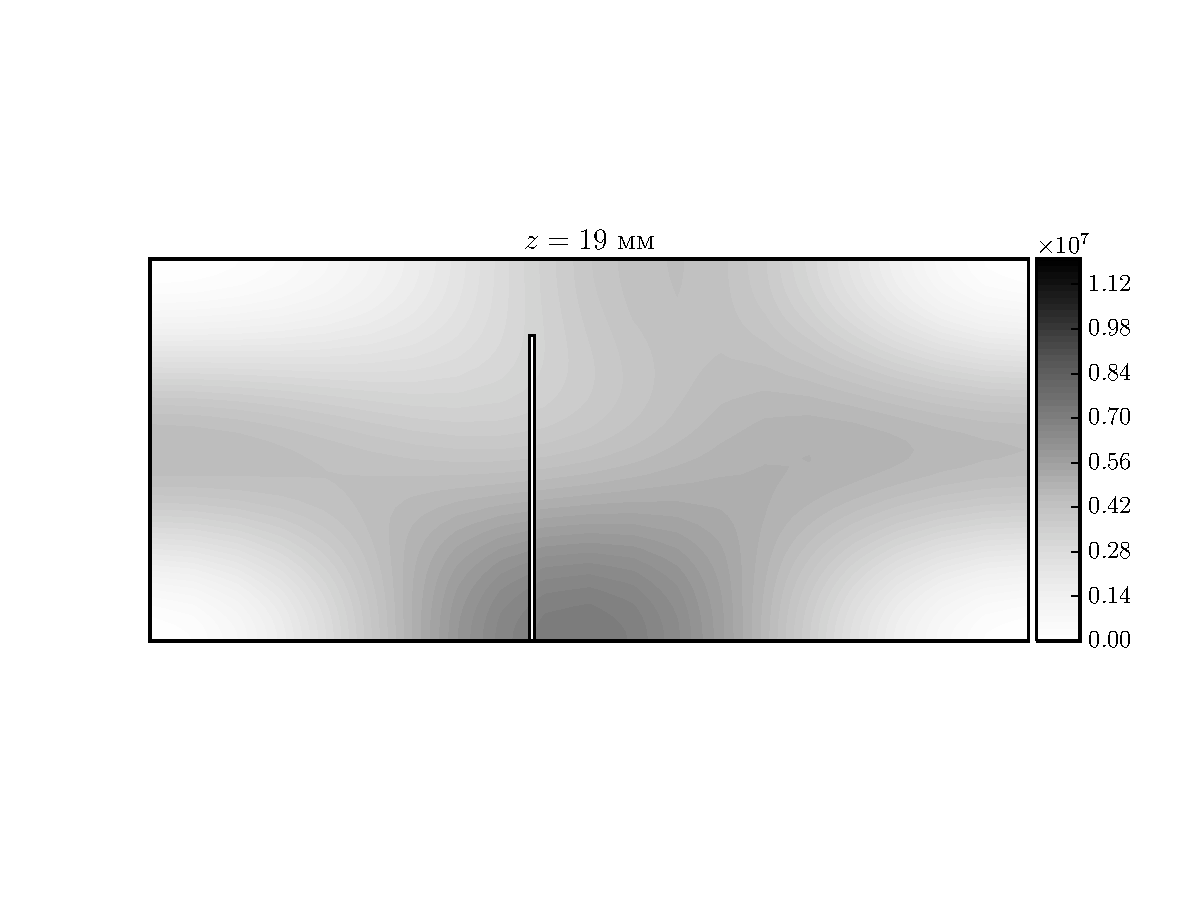
\includegraphics[width=.5\textwidth]{19}
		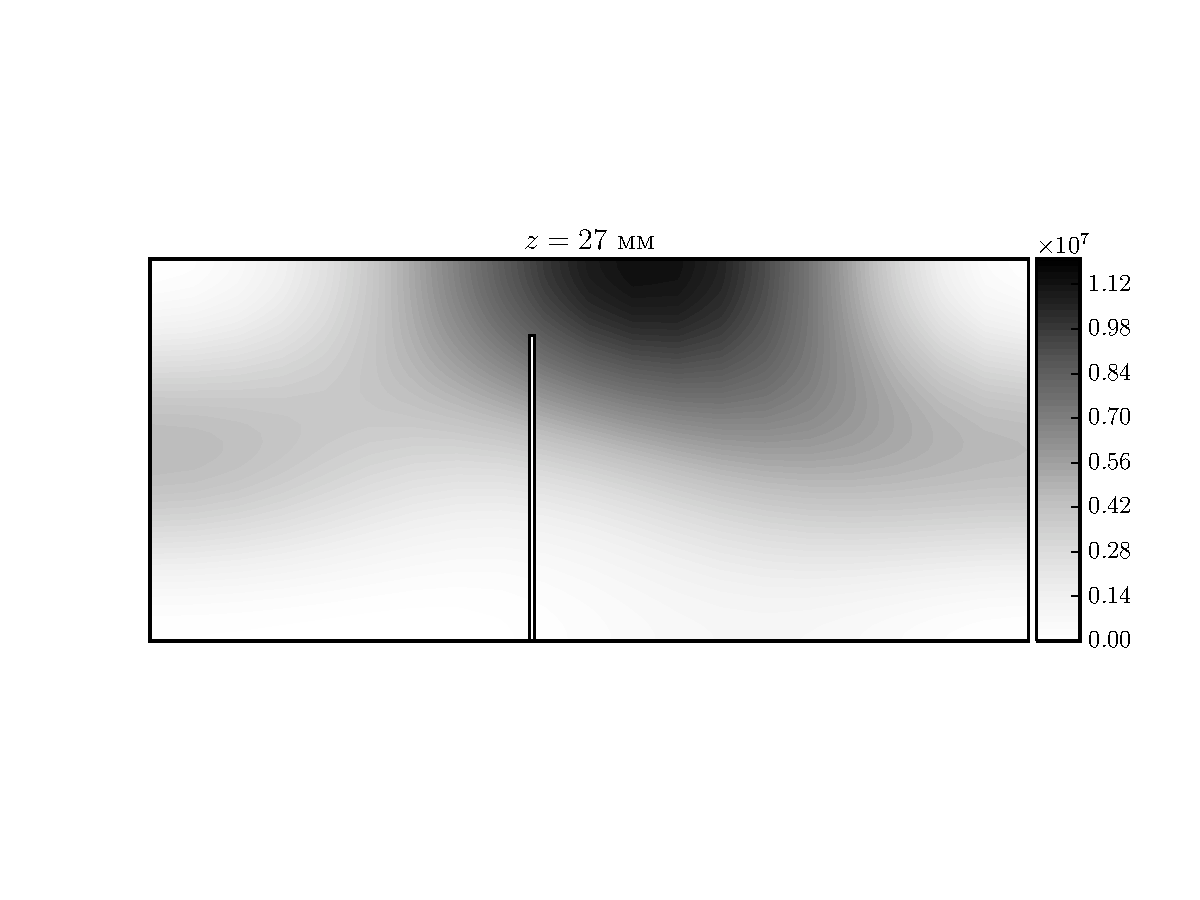
\includegraphics[width=.5\textwidth]{27}\hfil
		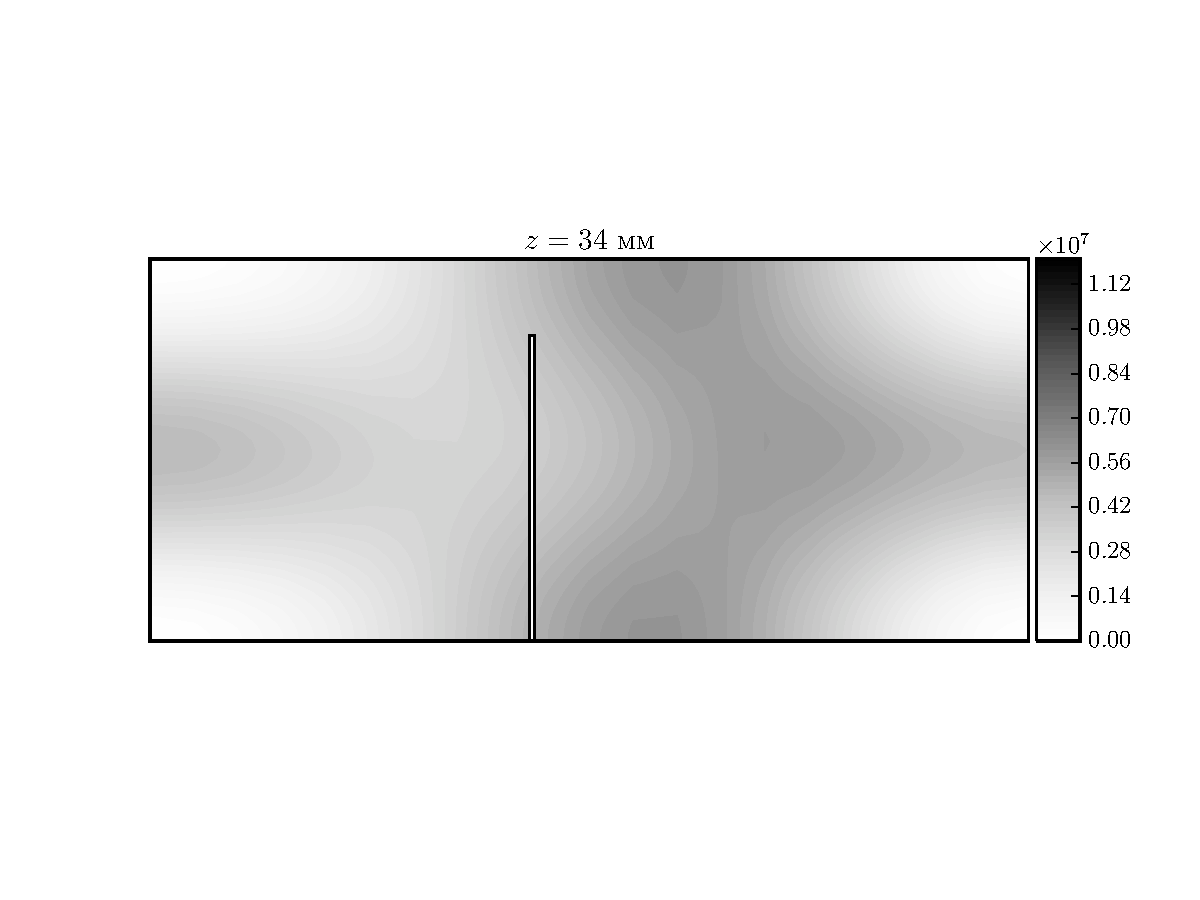
\includegraphics[width=.5\textwidth]{34}
		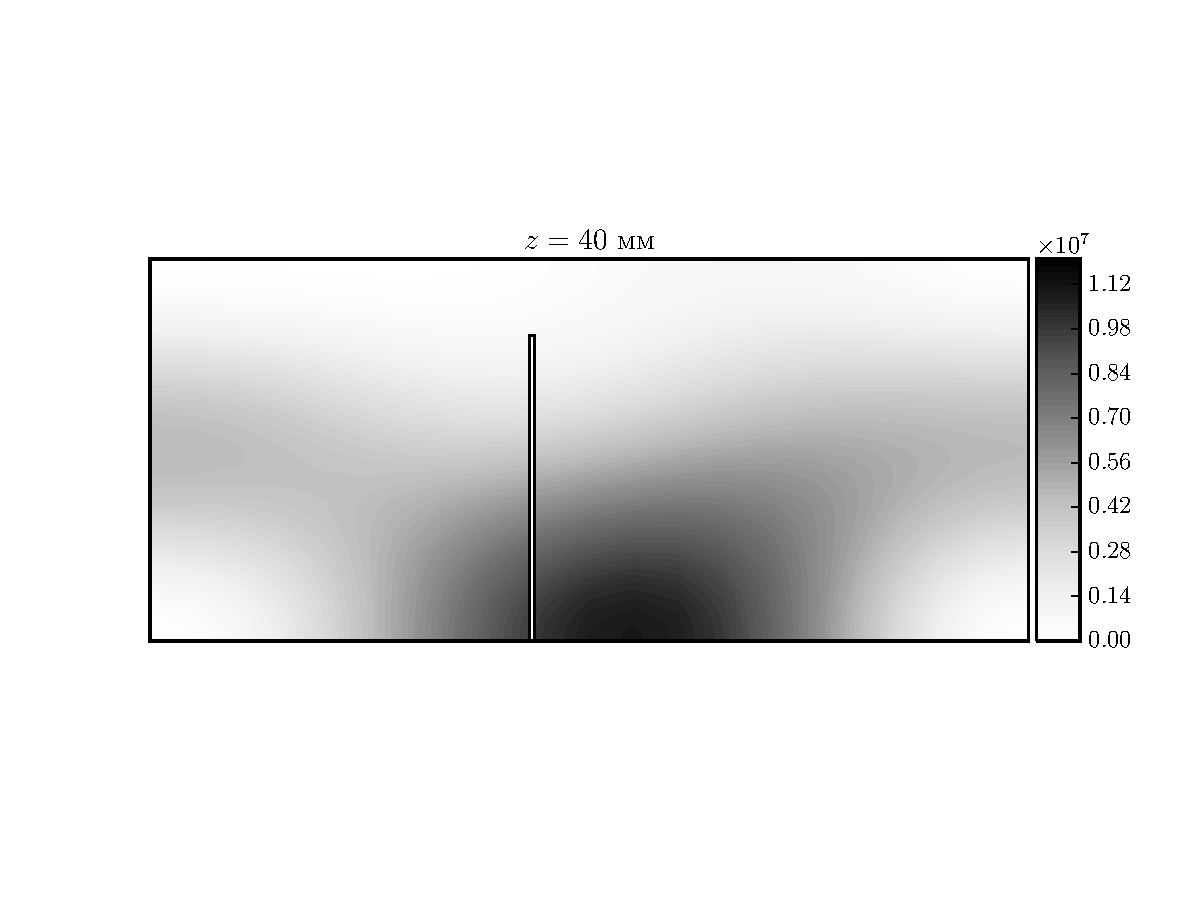
\includegraphics[width=.5\textwidth]{40}\hfil
		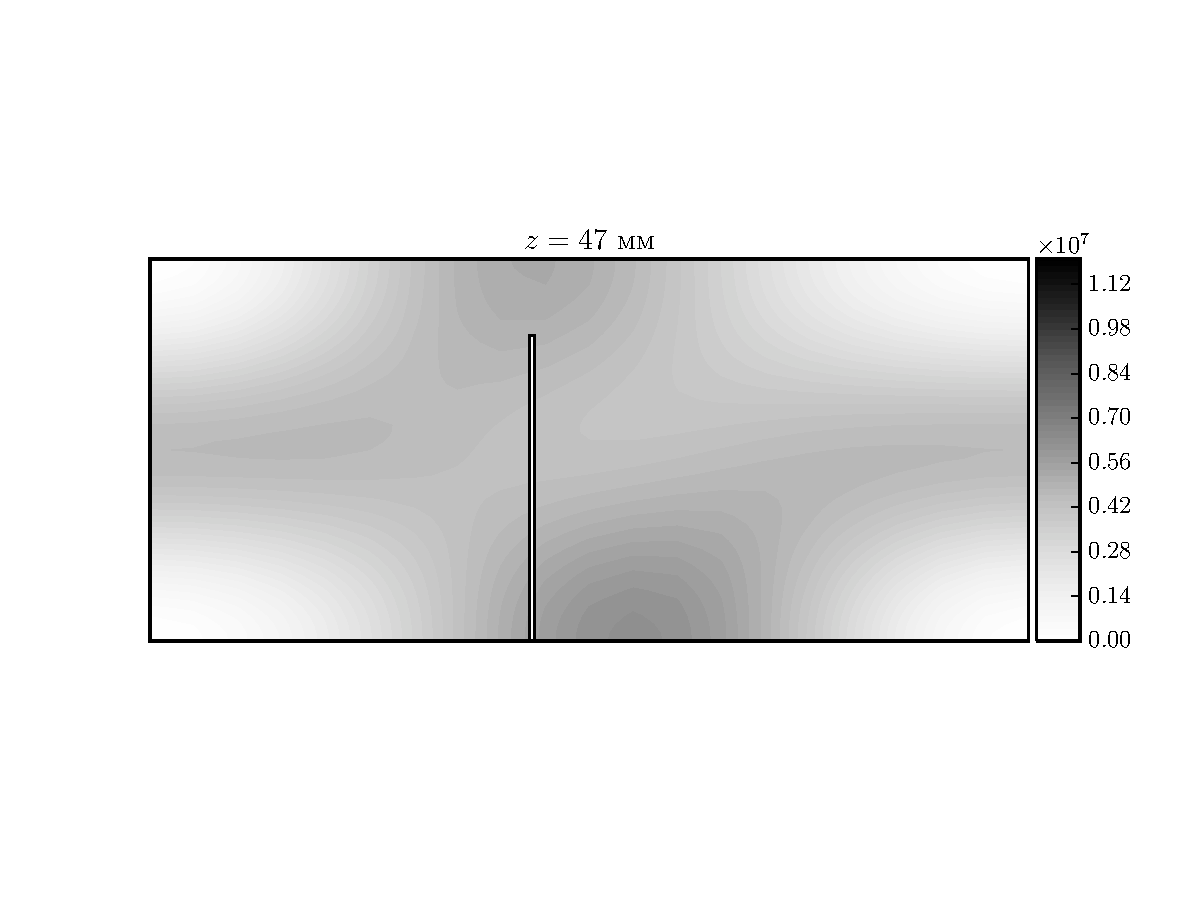
\includegraphics[width=.5\textwidth]{47}
		\caption{Распределение мощности в поперечном сечении}
	\end{figure}
\end{document}